\chapter{Introduction}

When using DSP for sound design, whether it be software instruments, audio effects or any other kind of creative or
practical sound processing, the program can usually be expressed as a pipeline, or composition of common, reusable
blocks. These blocks could be anything from filters and delay lines to envelopes and oscillators, with a rich tappestry
of algorithms in between, but most audio processing programs use the from the same set of basic, well known blocks, and
then work with composition \todo{continue}

\section{Audio Processing}

Audio is usually represented as a stream of samples, each either a floating or fixed point number, and for processing,
the stream is split up into buffers of a fixed size. In most normal applications, the samples are 16, 24 or 32 bits, at
sample rates of anywhere from 44.1kHz to 192kHz. Buffer sizes vary a lot depending on the real time requirements, from
as low as 16 samples up to 4096. Larger buffers usually allow for better performance, while increasing the processing
latency.

When dealing with multiple channels in one stream, such as would be the case for stereo or surround sound, the samples
from each channel are usually interleaved, forming buffers of frames of samples (see \autoref{fig:buffersframes}).
These buffers are then passed to a processing callback one at a time by the host audio system, whether that is the OS
directly, or in the case of audio plugins, the plugin host application. This asynchronous callback-based model is what
is used by most real time audio frameworks, such as ALSA, Jack, VST

\begin{figure}
  \includestandalone[width=\textwidth]{Pictures/framevsbuffer}
  \caption{A stereo audio signal broken into buffers of 8 frames of two samples each.}
  \label{fig:buffersframes}
\end{figure}

\begin{lstlisting}[language=c++,label=lst:jackmerge,float,caption={
    An example process function that sends one input channel to two output channels. Numbers of channels are determined before registering the process function.
}]
int process(float* input, float* output, unsigned nframes) {
  for (int i = 0; i < nframes; i++) {
    output[i * 2] = input[i];
    output[0 * 2 + 1] = input[i];
  }
}
\end{lstlisting}

\section{The Problem}
\todo{At a High level, which issues are the existing solutions trying to solve, and what do i want to solve?}

In many cases audio processing is being done live, and has hard real-time requirements. As an example, when processing
a stereo signal with a sample rate of \SI{44.1}{kHz}, one has to be able to process \num{88200} samples per second,
which leaves around \SI{11.3}{\micro\second} per sample. For this reason, DSP code is usually written in a low-level
high-performing language, like C or C++. However, as mentioned before designing audio processing is inherintly a
largely compositional process, in which one rarely needs to worry about individual samples, buffer sizes,
representation as fixed or floating point etc, except when implementing the low level components that make up the
pipeline.

\todo{What exact code do  i want to be able to write?} \\
\todo{Set goals/constraints for evaluation} \\
\todo{Evaluation: Performance and comparisons of examples} \\

\section{The Example}

As a case study, i will be using a very simple echo effect. It takes a single channel of input, which is delayed by
some amount of samples, fed through a single-pole IIR ladder filter, decreased in gain, and fed back into the input to
be delayed again. This can be seen in \autoref{fig:echoblock}

\begin{figure}
  \centering
  \includestandalone[width=\textwidth]{Pictures/block_echo}
  \caption{Block diagram of the echo effect.}
  \label{fig:echoblock}
\end{figure}

\begin{lstlisting}[language=faust,label=lst:faustecho,caption={
    Simple echo effect in faust, with time control, a 1-pole IIR filter, feedback gain and a dry/wet mix control. Paste into \url{https://faustide.grame.fr} to run the example.
}]
time_samples = 11025;
filter_a = 0.9;
feedback = 1.0; 
dry_wet_mix = 0.5;

filter = (((_ * filter_a, _ * (1 - filter_a)) : + ) ~ _);
echo = (+ : @(time_samples)) ~ (filter * feedback);
process = _ <: (echo * dry_wet_mix) + (_ * (1 - dry_wet_mix));
\end{lstlisting}

\begin{figure}
  \centering
  \def\svgwidth{\columnwidth}
  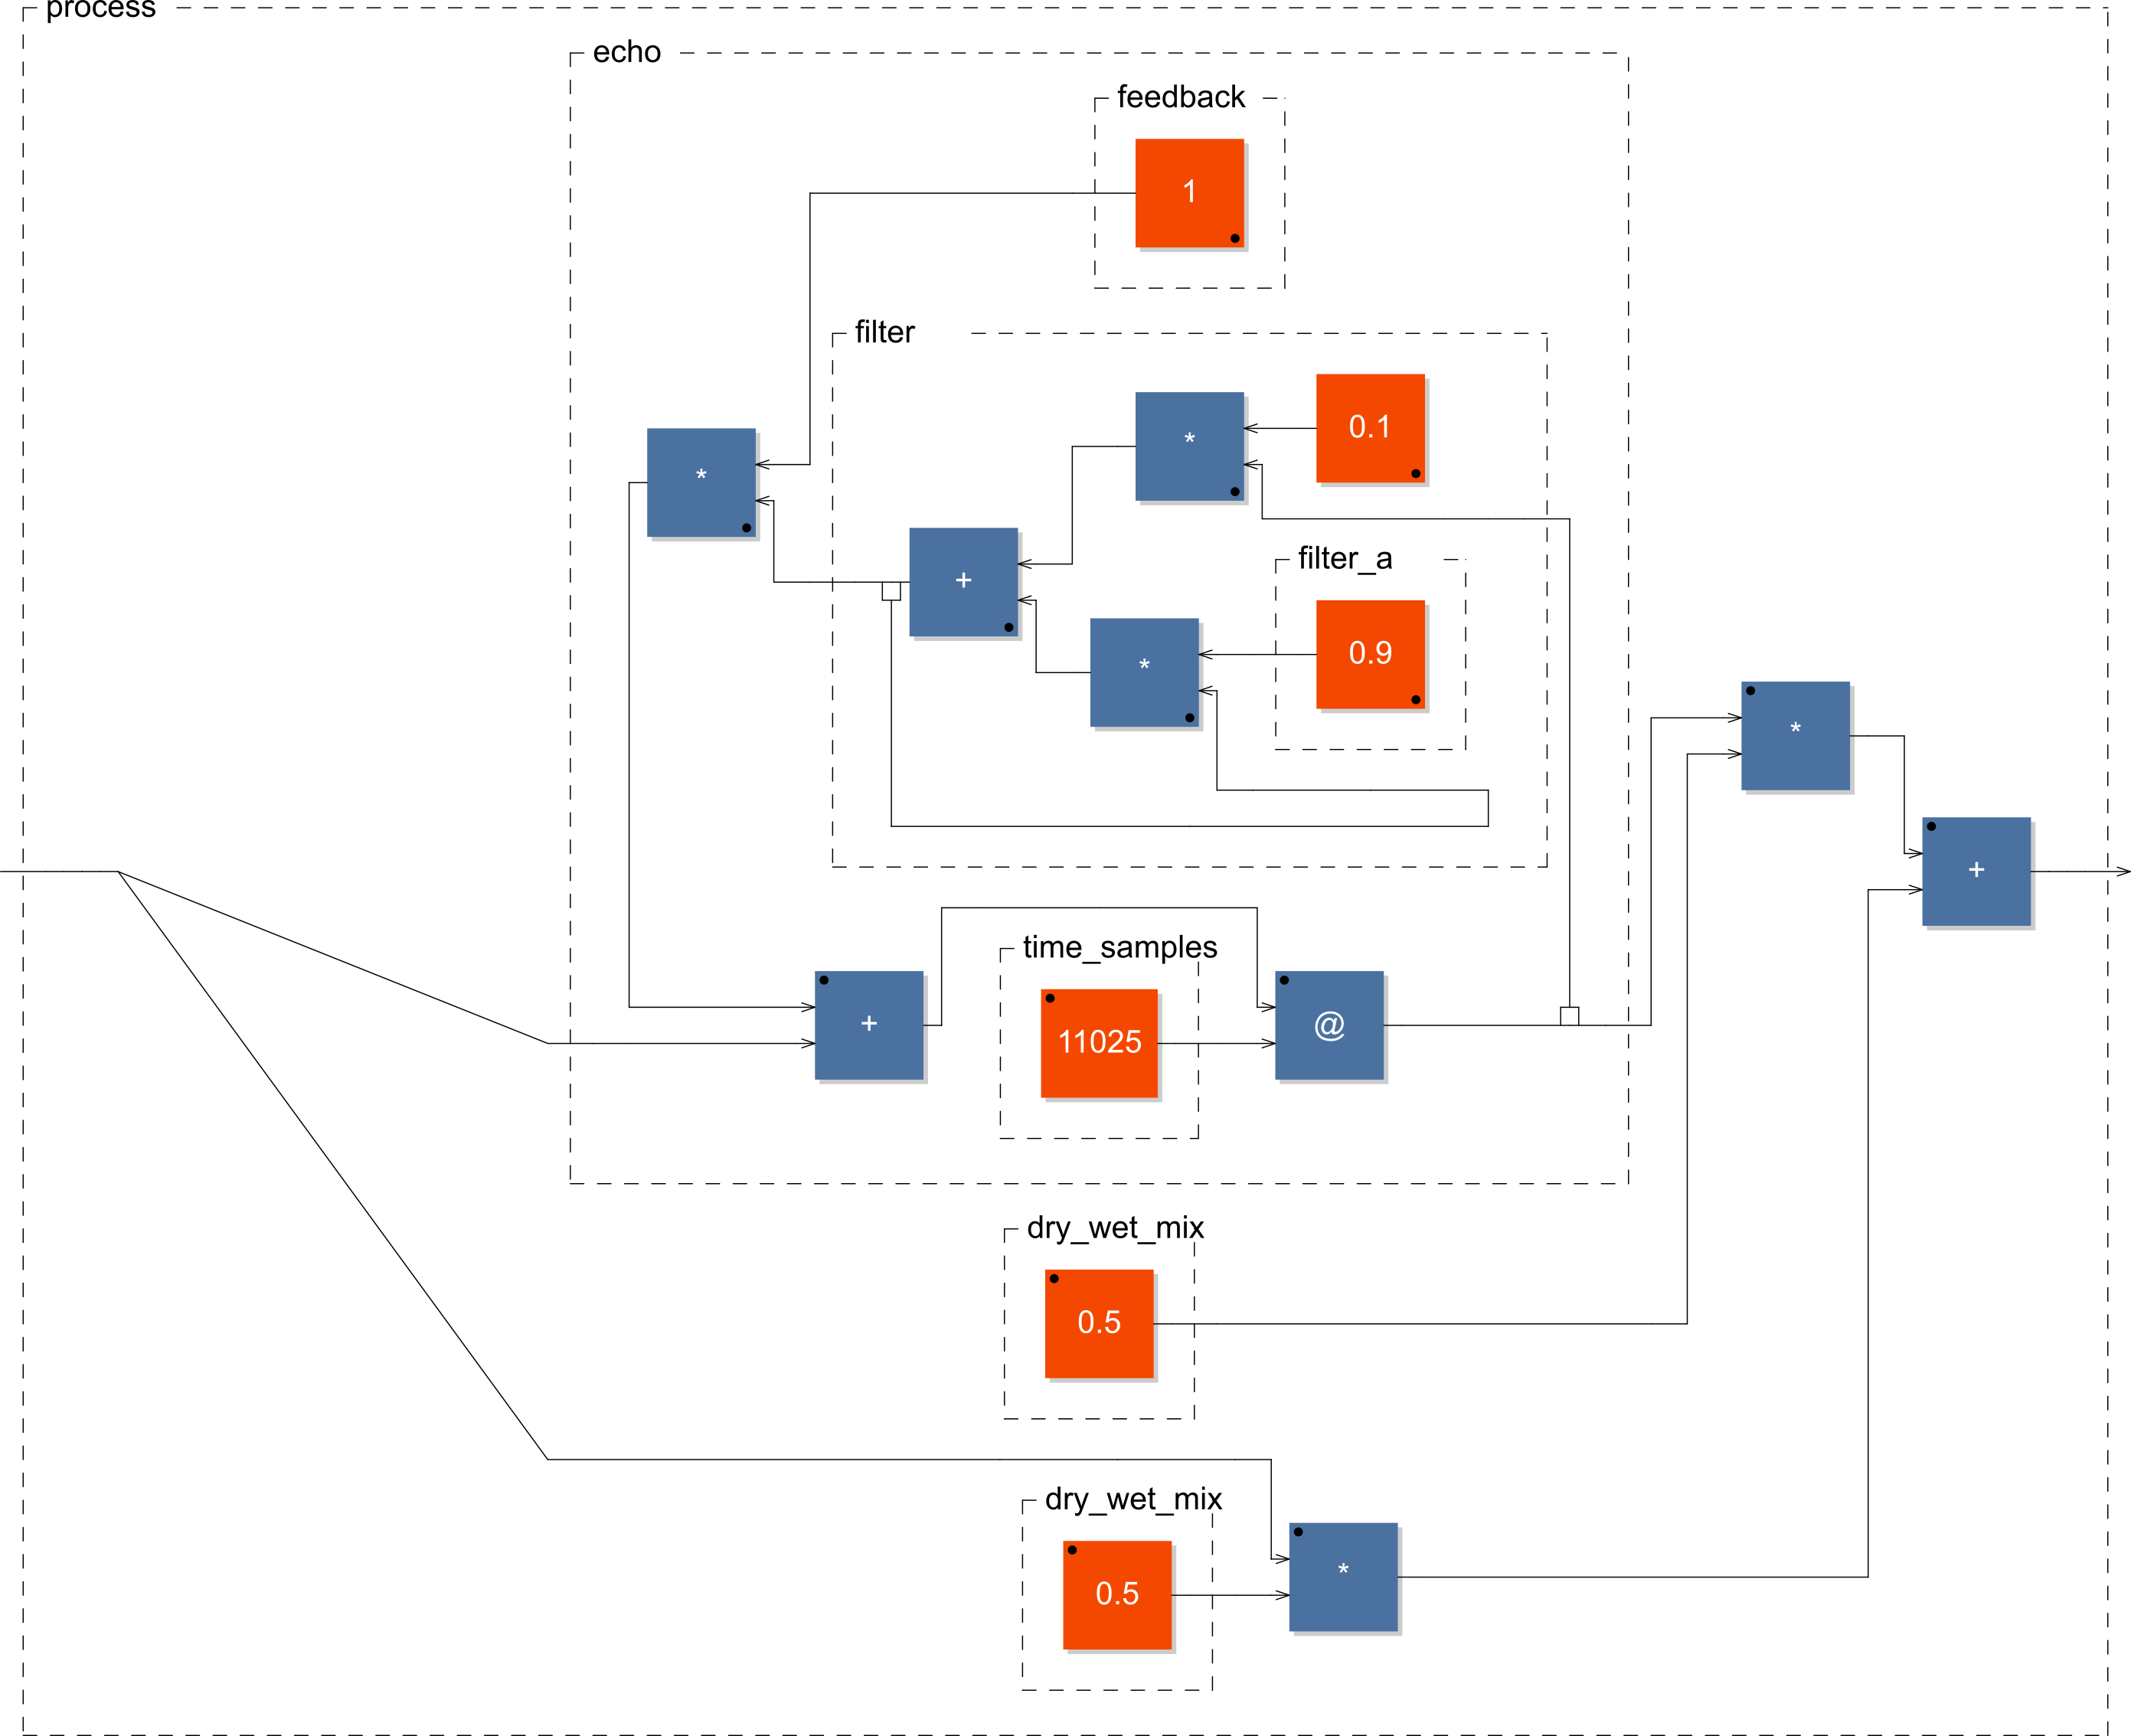
\includegraphics[width=\textwidth]{faustecho.png}
  \caption{Block diagram generated by faust for code in \autoref{lst:faustecho}}
  \label{fig:faustecho}
\end{figure}
